% !TEX root = ../../prj4projektdokumentation.tex
\chapter{Metode}


Til gennemførelse af dette projekt er ASE-modellen blevet anvendt som udgangspunkt. Denne model viser de forskellige faser, projektgruppen skal igennem på vejen mod et endeligt produkt og en veldokumenteret og gennemarbejdet rapport. ASE-modellen ses på figur \ref{fig:Asemodel} Gruppen har desuden anvendt en iterativ og empirisk arbejdsmetode. Der er brugt faglitteratur og teori fra undervisningen til at danne vidensgrundlag for projektet om spændingsregulatoren. Undervejs er der indsamlet nye erfaringer i forbindelse med udviklingen af produktet. 
I udviklingsfasen er der anvendt SysML og UML, der sammen med Use Casene har givet overblik over systemet både grafisk og skriftligt. Dette har dannet grundlag for opbygningen af systemet. 

\begin{figure}[H] 
	\centering
	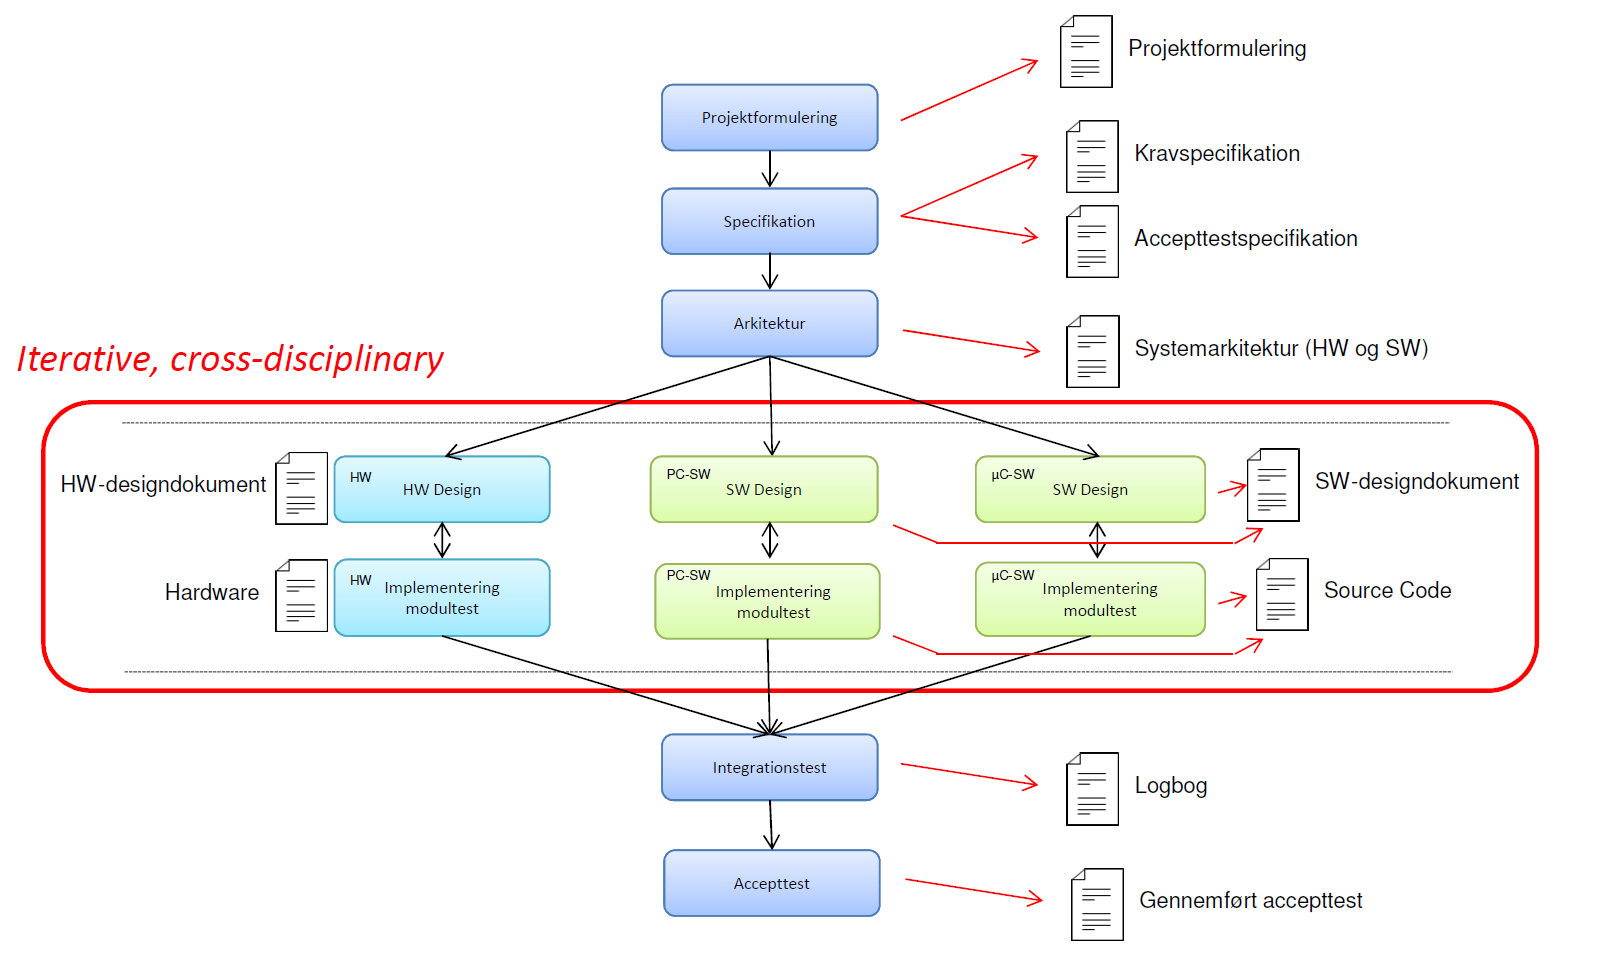
\includegraphics[width=0.7\textwidth]{Figure/Asemodel}
	\caption{Asemodellen}
	\label{fig:Asemodel}
\end{figure}

For at styre og lede projektet har gruppen ladet sig inspirere af Scrum principperne. Fra starten af projektet har gruppen oprettet sprints og defineret dertilhørende opgaver. Gruppen har ikke afholdt daily scrums, men har gennemsnitligt haft 1-2 ugentlige gruppemøder, samt ugentligt vejledermøde. Dette har medført en jævn arbejdsgang og et godt flow i projektet. 